\chapter{方法与研究设计}
\label{chap:method}

\section{方法概述}

在本章说明研究对象、数据来源、实验条件或理论推导过程。图、表和公式应在正文中先被引用，再出现于相邻位置。图~\ref{fig:single-plot} 使用了模板自带的 PNG 示例文件，实际写作时请用自己的图片替换它。

\begin{equation}
  y_i = \alpha x_i + \beta + \varepsilon_i,
  \label{eq:linear-model}
\end{equation}

式~\eqref{eq:linear-model} 是公式编号与交叉引用的示例。行内公式写作 $y=f(x)$；只对需要单独讨论或在后文引用的公式使用 \texttt{equation} 环境。

彼此关联的多行推导可使用 \texttt{align} 环境，并只给需要引用的行添加标签：

\begin{align}
  \hat{y}_i &= \alpha x_i + \beta, \label{eq:prediction} \\
  \mathcal{L} &= \sum_{i=1}^{n}\left(y_i-\hat{y}_i\right)^2.
  \label{eq:loss}
\end{align}

式~\eqref{eq:prediction} 和式~\eqref{eq:loss} 分别给出预测值与示例损失函数。

\begin{figure}[htbp]
  \centering
  % Omit the extension so the same source can be supplied as PDF, PNG, or JPG.
  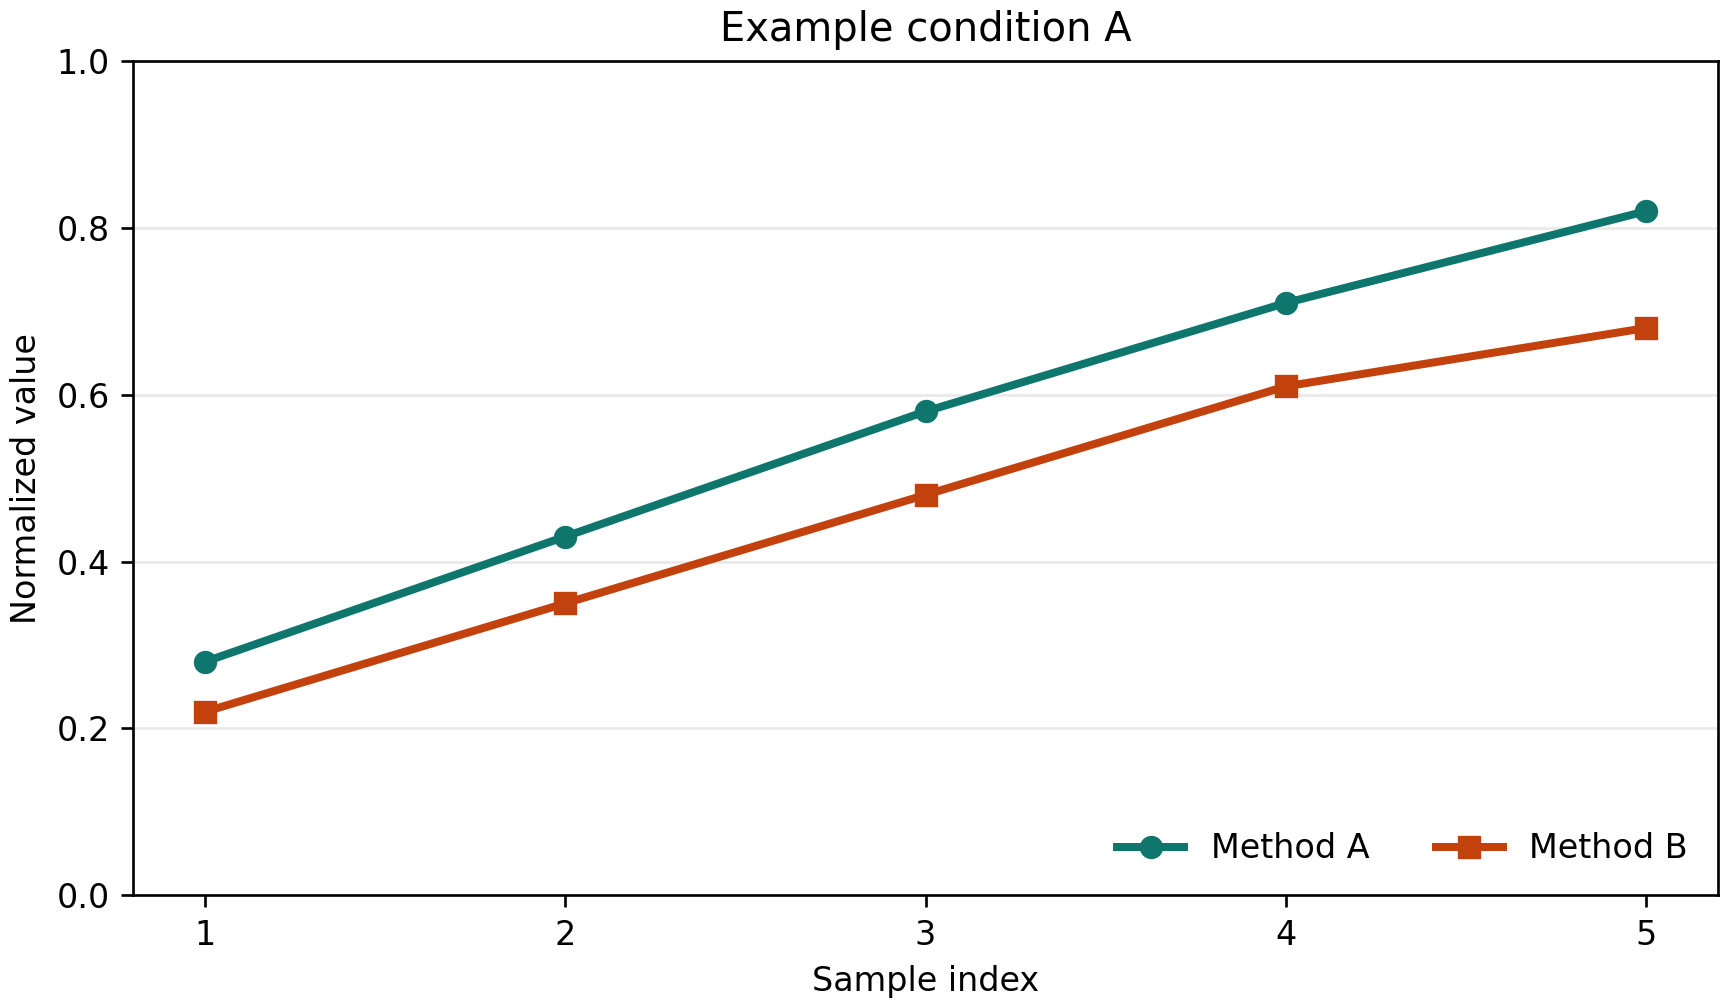
\includegraphics[width=0.74\textwidth]{example-plot-a}
  % 方括号内为插图清单中的独立名称，花括号内为正文图题。
  \caption[示例单图]{示例单图：请用自己的图片和说明替换}
  \label{fig:single-plot}
\end{figure}

\section{概念、定理与证明}

需要正式定义、定理或证明时，可直接使用类文件已提供的环境。

\begin{definition}[示例定义]
设 $\mathcal{D}$ 是研究对象的样本集合。若一个指标可以由 $\mathcal{D}$ 唯一计算，则称该指标在本研究设定下是可观测的。
\end{definition}

\begin{theorem}[示例命题]
若 $\varepsilon_i=0$ 且 $\alpha\ne0$，则式~\eqref{eq:linear-model} 中的 $x_i$ 可由 $y_i$ 唯一确定。
\label{thm:invertible-example}
\end{theorem}

\begin{proof}
由式~\eqref{eq:linear-model} 可得 $x_i=(y_i-\beta)/\alpha$。由于 $\alpha\ne0$，该表达式唯一，命题成立。
\end{proof}

定理~\ref{thm:invertible-example} 仅展示排版方式；最终论文应保留与研究内容有关且经过完整论证的定义和定理。

\begin{table}[htbp]
  \centering
  \caption{示例结果表}
  \label{tab:example}
  \begin{tabular}{lcc}
    \toprule
    方法 & 指标一 & 指标二 \\
    \midrule
    方法 A & 0.00 & 0.00 \\
    方法 B & 0.00 & 0.00 \\
    \bottomrule
  \end{tabular}
\end{table}

表~\ref{tab:example} 展示了三线表示例。需要插图时，将图像放在 \texttt{figures/} 目录，并使用 \verb|\includegraphics| 插入。
